\documentclass[11pt,compress,t,notes=noshow, xcolor=table]{beamer}


\input{../../style/preamble}
\input{../../latex-math/basic-math}
\input{../../latex-math/basic-ml}

\title{Optimization in Machine Learning}

\begin{document}

\titlemeta{% Chunk title (example: CART, Forests, Boosting, ...), can be empty
  First order methods
  }{% Lecture title  
  Comparison of first order methods
  }{% Relative path to title page image: Can be empty but must not start with slides/
  figure_man/linesearch.png
  }{
    \item Gradient Descent
    \item Stochastic Gradient Descent
    \item Momentum
    \item Step size control
}


\begin{vbframe}{Comparison of first order methods}
Comparison of (S)GD, (S)GD + momentum, and (S)GD + momentum + step size control on simulated data:

\begin{itemize}
    \item Linear regression (squared loss) simulation $\bm{Y} = \bm{X}\thetav^{\ast} + \bm{\varepsilon}$ with $n=500$ samples and $p=11$ features, where $\thetav^{\ast}=(-5,-4,\ldots,4,5)^{\top}$, $\bm{\varepsilon} \sim \mathcal{N}(\bm{0}, \bm{I})$, and $\bm{X} \sim \mathcal{N}(\bm{0}, \Sigma)$ for $\Sigma=\bm{I}$ (indep. features) or $\Sigma_{i,j}=0.9^{|i-j|}$ (corr. features)
    \item Indep. features result in a condition number of $\approx 2.9$, whereas the corr. feature set-up produces a bad condition number of $\approx 94$
    \item We set the momentum parameter to $\texttt{momentum}=0.5$
    \item The step size $\alpha^{[t]}$ is decayed exponentially using deterministic schedule $\alpha^{[t]}=\alpha^{[0]} \cdot \texttt{decay}^{t/t_{\text{max}}}$ for $\texttt{decay}=0.05$
    \item For GD and SGD we use 3 step sizes each (low, medium, large) to illustrate the effect of $\alpha$, $\texttt{momentum}$ and $\texttt{decay}$.
    \item ERM has unique global minimizer given by $\thetah = (\bm{X}^{\top}\bm{X})^{-1}\bm{X}^{\top} \bm{Y}$
    \item We also track the estimation error $\Vert \thetav - \thetav^{\ast} \Vert_2$
\end{itemize}

\end{vbframe}

%%%% GD linear

\begin{vbframe}{Lin-Reg (GD + small step size)}
\vspace{-0.4cm}
GD with small $\alpha=2\cdot10^{-4}$ and indep. features:
\begin{figure}
            \includegraphics[width=0.8\textwidth]{slides/04-multivariate-first-order/figure_man/simu_linmod/GD_reg_small_lr_iters.pdf} \\
             \includegraphics[width=0.8\textwidth]{slides/04-multivariate-first-order/figure_man/simu_linmod/GD_reg_coef_small.pdf}\\
            \begin{footnotesize}
                Dashed line in test loss indicates irreducible error due to $\sigma=1$
            \end{footnotesize}
\end{figure}
Only momentum permits optim close to global min in $t_{\text{max}}=10000$ iters. Decay worsens performance as $\alpha$ was already too low.
\end{vbframe}

\begin{vbframe}{Lin-Reg (GD + med step size)}
\vspace{-0.4cm}
GD with medium $\alpha=2\cdot10^{-3}$ and indep. features:
\begin{figure}
            \includegraphics[width=0.8\textwidth]{slides/04-multivariate-first-order/figure_man/simu_linmod/GD_reg_med_lr_iters.pdf} \\
             \includegraphics[width=0.8\textwidth]{slides/04-multivariate-first-order/figure_man/simu_linmod/GD_reg_coef_med.pdf}\\
            \begin{footnotesize}
                Dashed line in test loss indicates irreducible error due to $\sigma=1$
            \end{footnotesize}
\end{figure}
Momentum accelerates optimization but all versions converge to global min. Decay slows down progress.
\end{vbframe}

\begin{vbframe}{Lin-Reg (GD + large step size)}
\vspace{-0.5cm}
GD with large $\alpha=1.4$ and indep. features:
\begin{figure}
            \includegraphics[width=0.8\textwidth]{slides/04-multivariate-first-order/figure_man/simu_linmod/GD_reg_large_lr_iters.pdf} \\
             \includegraphics[width=0.8\textwidth]{slides/04-multivariate-first-order/figure_man/simu_linmod/GD_reg_coef_large.pdf}\\
            \begin{footnotesize}
                Dashed line in test loss indicates irreducible error due to $\sigma=1$
            \end{footnotesize}
\end{figure}
Super fast convergence in $<20$ steps. Decay here speeds up optim. Coefficient paths show ``overshooting'' and oscillation at beginning.
\end{vbframe}

\begin{vbframe}{Lin-Reg (GD + corr. features)}
\vspace{-0.4cm}
GD with medium $\alpha=2\cdot10^{-3}$ and bad conditioning (corr. features):
\begin{figure}
            \includegraphics[width=0.8\textwidth]{slides/04-multivariate-first-order/figure_man/simu_linmod/GD_reg_med_lr_corr_iters.pdf} \\
             \includegraphics[width=0.8\textwidth]{slides/04-multivariate-first-order/figure_man/simu_linmod/GD_reg_coef_med_corr.pdf}\\
            \begin{footnotesize}
                Dashed line in test loss indicates irreducible error due to $\sigma=1$
            \end{footnotesize}
\end{figure}
Only plain GD and momentum converge in $t_{\text{max}}=10000$ iterations. Step size decay slows down optimization (non-convergence).
\end{vbframe}

%%% SGD linear

\begin{vbframe}{Lin-Reg (SGD + small step size)}
\vspace{-0.4cm}
SGD with small $\alpha=2\cdot10^{-4}$ and indep. features:
\begin{figure}
            \includegraphics[width=0.8\textwidth]{slides/04-multivariate-first-order/figure_man/simu_linmod/SGD_reg_small_lr_iters.pdf} \\
             \includegraphics[width=0.8\textwidth]{slides/04-multivariate-first-order/figure_man/simu_linmod/SGD_reg_coef_small.pdf}\\
            \begin{footnotesize}
                Dashed line in test loss indicates irreducible error due to $\sigma=1$
            \end{footnotesize}
\end{figure}
Only momentum permits optim close to global min in $t_{\text{max}}=10000$ iters. Decay again worsens performance. Coef paths $\approx$ smooth. 
\end{vbframe}

\begin{vbframe}{Lin-Reg (SGD + med step size)}
\vspace{-0.4cm}
SGD with medium $\alpha=1\cdot10^{-3}$ and indep. features:
\begin{figure}
            \includegraphics[width=0.8\textwidth]{slides/04-multivariate-first-order/figure_man/simu_linmod/SGD_reg_med_lr_iters.pdf} \\
             \includegraphics[width=0.8\textwidth]{slides/04-multivariate-first-order/figure_man/simu_linmod/SGD_reg_coef_med.pdf}\\
            \begin{footnotesize}
                Dashed line in test loss indicates irreducible error due to $\sigma=1$
            \end{footnotesize}
\end{figure}
Momentum accelerates optim but all variants except decay converge. Coef paths slightly jittered.
\end{vbframe}

\begin{vbframe}{Lin-Reg (SGD + large step size)}
\vspace{-0.4cm}
SGD with large $\alpha=1 \cdot 10^{-2}$ and indep. features:
\begin{figure}
            \includegraphics[width=0.8\textwidth]{slides/04-multivariate-first-order/figure_man/simu_linmod/SGD_reg_large_lr_iters.pdf} \\
             \includegraphics[width=0.8\textwidth]{slides/04-multivariate-first-order/figure_man/simu_linmod/SGD_reg_coef_large.pdf}\\
            \begin{footnotesize}
                Dashed line in test loss indicates irreducible error due to $\sigma=1$
            \end{footnotesize}
\end{figure}
Only variants with decay converge. Loss and coef paths very noisy and decay mandatory for noise to disappear.
\end{vbframe}

\begin{vbframe}{Lin-Reg (SGD + corr. features)}
\vspace{-0.4cm}
SGD with medium $\alpha=1\cdot10^{-3}$ and bad conditioning (corr. features):
\begin{figure}
            \includegraphics[width=0.8\textwidth]{slides/04-multivariate-first-order/figure_man/simu_linmod/SGD_reg_med_lr_corr_iters.pdf} \\
             \includegraphics[width=0.8\textwidth]{slides/04-multivariate-first-order/figure_man/simu_linmod/SGD_reg_coef_med_corr.pdf}\\
            \begin{footnotesize}
                Dashed line in test loss indicates irreducible error due to $\sigma=1$
            \end{footnotesize}
\end{figure}
Only SGD+mom. converges in $t_{\text{max}}=10000$ and achieves generalization. Decay slows down while momentum accelerates optim.
\end{vbframe}

\begin{vbframe}{Comparison of first order methods}
Comparison of (S)GD, (S)GD + momentum, and (S)GD + momentum + step size control on simulated data:

\begin{itemize}
    \item Logistic regression (cross-entropy loss) simulation also with $n=500$ samples and $p=11$ features, where $\thetav^{\ast}=(-5,-4,\ldots,4,5)^{\top}$ and $\bm{X} \sim \mathcal{N}(\bm{0}, \Sigma)$ for $\Sigma=\bm{I}$ (indep. features) or $\Sigma_{i,j}=0.9^{|i-j|}$ (corr. features)
    \item To simulate response, we set $y^{(i)} \sim \mathcal{B}(\pi^{(i)}), \pi^{(i)} = \frac{1}{1+e^{-(\bm{x}^{(i)})^{\top}\thetav^{\ast}}}$
    \item Indep. features again result in low condition number, whereas corr. features result in bad condition number
    \item We set the momentum parameter to $\texttt{momentum}=0.5$ and $\texttt{decay}=0.05$
    \item For GD and SGD we use 3 step sizes each (low, appropriate, large) to illustrate the effect of $\alpha$, $\texttt{momentum}$ and $\texttt{decay}$.
    \item ERM has unique global minimizer but no closed-form solution
    \item We also track the estimation error $\Vert \thetav - \thetav^{\ast} \Vert_2$
\end{itemize}

\end{vbframe}

%%% GD logistic

\begin{vbframe}{Log-Reg (GD + small step size)}
\vspace{-0.4cm}
GD with small $\alpha=2\cdot10^{-3}$ and indep. features:
\begin{figure}
            \includegraphics[width=0.8\textwidth]{slides/04-multivariate-first-order/figure_man/simu_linmod/GD_log_small_lr_iters.pdf} \\
             \includegraphics[width=0.8\textwidth]{slides/04-multivariate-first-order/figure_man/simu_linmod/GD_log_coef_small.pdf}\\
            \begin{footnotesize}
                Dashed line in test loss indicates irreducible error due to $\sigma=1$
            \end{footnotesize}
\end{figure}
No method converges in $t_{\text{max}}=10000$, as small updates keep the process in high-error regions, accumulating error over time.
\end{vbframe}

\begin{vbframe}{Log-Reg (GD + med step size)}
\vspace{-0.4cm}
GD with medium $\alpha=5\cdot10^{-2}$ and indep. features:
\begin{figure}
            \includegraphics[width=0.8\textwidth]{slides/04-multivariate-first-order/figure_man/simu_linmod/GD_log_med_lr_iters.pdf} \\
             \includegraphics[width=0.8\textwidth]{slides/04-multivariate-first-order/figure_man/simu_linmod/GD_log_coef_med.pdf}\\
            \begin{footnotesize}
                Dashed line in test loss indicates irreducible error due to $\sigma=1$
            \end{footnotesize}
\end{figure}
Momentum accelerates optimization while other versions still do not converge to global min. Decay slows down progress.
\end{vbframe}

\begin{vbframe}{Log-Reg (GD + large step size)}
\vspace{-0.5cm}
GD with large $\alpha=10$ and indep. features:
\begin{figure}
            \includegraphics[width=0.8\textwidth]{slides/04-multivariate-first-order/figure_man/simu_linmod/GD_log_large_lr_iters.pdf} \\
             \includegraphics[width=0.8\textwidth]{slides/04-multivariate-first-order/figure_man/simu_linmod/GD_log_coef_large.pdf}\\
            \begin{footnotesize}
                Dashed line in test loss indicates irreducible error due to $\sigma=1$
            \end{footnotesize}
\end{figure}
Super fast convergence for momentum around $30$ steps. Coefficient paths show ``overshooting'', while decay helps.
\end{vbframe}

\begin{vbframe}{Log-Reg (GD + corr. features)}
\vspace{-0.4cm}
GD with medium $\alpha=5\cdot10^{-2}$ and bad conditioning (corr. features):
\begin{figure}
            \includegraphics[width=0.8\textwidth]{slides/04-multivariate-first-order/figure_man/simu_linmod/GD_log_med_lr_corr_iters.pdf} \\
             \includegraphics[width=0.8\textwidth]{slides/04-multivariate-first-order/figure_man/simu_linmod/GD_log_coef_med_corr.pdf}\\
            \begin{footnotesize}
                Dashed line in test loss indicates irreducible error due to $\sigma=1$
            \end{footnotesize}
\end{figure}
Only GD with momentum converge in $t_{\text{max}}=10000$ iterations. Step size decay slows down optimization (non-convergence).
\end{vbframe}


%%% SGD logistic

\begin{vbframe}{Log-Reg (SGD + small step size)}
\vspace{-0.4cm}
SGD with small $\alpha=2\cdot10^{-3}$ and indep. features:
\begin{figure}
            \includegraphics[width=0.8\textwidth]{slides/04-multivariate-first-order/figure_man/simu_linmod/SGD_log_small_lr_iters.pdf} \\
             \includegraphics[width=0.8\textwidth]{slides/04-multivariate-first-order/figure_man/simu_linmod/SGD_log_coef_small.pdf}\\
            \begin{footnotesize}
                Dashed line in test loss indicates irreducible error due to $\sigma=1$
            \end{footnotesize}
\end{figure}
No method converges since lr is too small. Decay makes it even worse. 
\end{vbframe}

\begin{vbframe}{Log-Reg (SGD + med step size)}
\vspace{-0.4cm}
SGD with medium $\alpha=5\cdot10^{-2}$ and indep. features:
\begin{figure}
            \includegraphics[width=0.8\textwidth]{slides/04-multivariate-first-order/figure_man/simu_linmod/SGD_log_med_lr_iters.pdf} \\
             \includegraphics[width=0.8\textwidth]{slides/04-multivariate-first-order/figure_man/simu_linmod/SGD_log_coef_med.pdf}\\
            \begin{footnotesize}
                Dashed line in test loss indicates irreducible error due to $\sigma=1$
            \end{footnotesize}
\end{figure}
Momentum accelerates optim but all variants except decay converge. Coef paths slightly jittered.
\end{vbframe}

\begin{vbframe}{Log-Reg (SGD + large step size)}
\vspace{-0.4cm}
SGD with large $\alpha=5 \cdot 10^{-1}$ and indep. features:
\begin{figure}
            \includegraphics[width=0.8\textwidth]{slides/04-multivariate-first-order/figure_man/simu_linmod/SGD_log_large_lr_iters.pdf} \\
             \includegraphics[width=0.8\textwidth]{slides/04-multivariate-first-order/figure_man/simu_linmod/SGD_log_coef_large.pdf}\\
            \begin{footnotesize}
                Dashed line in test loss indicates irreducible error due to $\sigma=1$
            \end{footnotesize}
\end{figure}
Only variants with simple decay converge, others overshoot severely. Loss and coef paths very noisy.
\end{vbframe}

\begin{vbframe}{Log-Reg (SGD + corr. features)}
\vspace{-0.4cm}
SGD with medium $\alpha=5\cdot10^{-2}$ and bad conditioning (corr. features):
\begin{figure}
            \includegraphics[width=0.8\textwidth]{slides/04-multivariate-first-order/figure_man/simu_linmod/SGD_log_med_lr_corr_iters.pdf} \\
             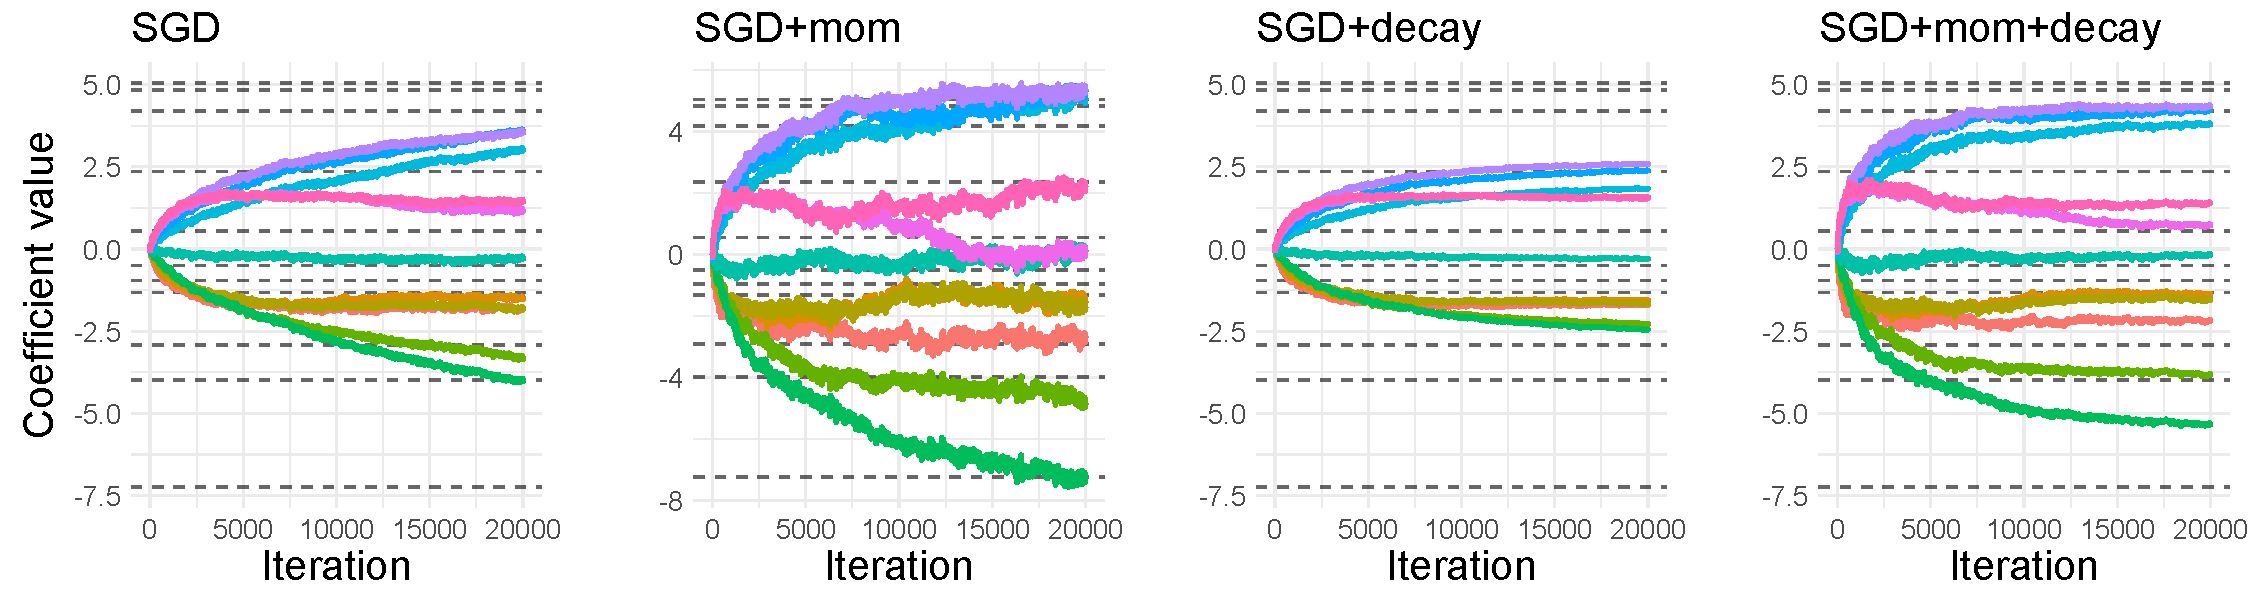
\includegraphics[width=0.8\textwidth]{slides/04-multivariate-first-order/figure_man/simu_linmod/SGD_log_coef_med_corr.pdf}\\
            \begin{footnotesize}
                Dashed line in test loss indicates irreducible error due to $\sigma=1$
            \end{footnotesize}
\end{figure}
Only SGD and SGD+mom converge in $t_{\text{max}}=10000$. Decay slows down while momentum accelerates optim.
\end{vbframe}


\endlecture
\end{document}

%%% 



%% 
